\section{Supplementary Material} 

\setcounter{table}{0}
\setcounter{figure}{0}
\renewcommand{\thetable}{SI\arabic{table}}
\renewcommand{\thefigure}{SI\arabic{figure}}

\subsection{Formula for Set Size}
To calculate the size of the different sets, we will use the binomial coefficients to calculate the possible combinations. The general form of the binominal coefficient is written as
\[\left( \begin{array}{c}
n \\ 
k \end{array}
\right)=\frac{n!}{k!\left(n-k\right)!}\] 

Where ``!'' is the factorial operator. So $n!=n\times \left(n-1\right)\times \left(n-2\right)\times \left(n-3\right)\times \dots \times 3\times 2\times 1$. One rule that is being used over and over again is the fact that we can rewrite the sum of binomial coefficients excluding the empty set (i.e. i=0) as 
\[\sum^n_{i=1}{\left( \begin{array}{c}
n \\ 
i \end{array}
\right)}=2^n-1\] 

When we need to calculate the size of each set, we need to split them into two different cases; one where we allow interactions without having main terms present, and the other where main terms should always follow the interaction. \\

\subsection{Case 1 – No Restriction}
\subsubsection{Ma} \hfill 

To calculate the size of the sets, we can use the binomial coefficient. Since the size of the set Ma will be all the combinations of the covariates. Let us denote the number of covariates with n. If we have an example with three covariates meaning n=3, then the combination of these where we have all three present can be written with the binomial coefficient as
\[\left( \begin{array}{c}
3 \\ 
3 \end{array}
\right)=\frac{3!}{3!\left(3-3\right)!}=1\] 
If only two covariates are to be present at the same time then the possible combinations become 
\[\left( \begin{array}{c}
3 \\ 
2 \end{array}
\right)=\frac{3!}{2!\left(3-2\right)!}=3\] 
And the same if only one should be present
\[\left( \begin{array}{c}
3 \\ 
1 \end{array}
\right)=\frac{3!}{1!\left(3-1\right)!}=3\] 
The final one is the one where no covariates are present
\[\left( \begin{array}{c}
3 \\ 
0 \end{array}
\right)=\frac{3!}{0!\left(3-0\right)!}=1\] 
Then the number of models in this set will be the sum of all these


\[\#models\ in\ Ma=\left( \begin{array}{c}
3 \\ 
3 \end{array}
\right)+\left( \begin{array}{c}
3 \\ 
2 \end{array}
\right)+\left( \begin{array}{c}
3 \\ 
1 \end{array}
\right)+\left( \begin{array}{c}
3 \\ 
0 \end{array}
\right)=\sum^3_{i=0}{\left( \begin{array}{c}
3 \\ 
i \end{array}
\right)}\] 
Using the rules from binomial coefficients, we can rewrite this into
\[\#models\ in\ Ma=\sum^3_{i=0}{\left( \begin{array}{c}
3 \\ 
i \end{array}
\right)}=\left(2^3\right)=8\] 
We can generalize this to the n covariates case with 
\[\#models\ in\ Ma=\sum^n_{i=1}{\left( \begin{array}{c}
n \\ 
i \end{array}
\right)}=\left(2^n\right)\] 

\subsubsection{Formally Written} \hfill \break 
\noindent Let X be the set of covariates 
\[X=\left.x_1,x_2,..,x_n\right.\] 
\[\left|X\right|=n\] 
\[\left|\mathcal{P}\left(X\right)\right|=2^n\] 


\noindent The set Ma is then the power set of H excluding the empty set
\[Ma=\left.S:S\subseteq X\right.\] 

Each element $S\in Ma$ is a set of the covariates e.g. $S=\left.x_3,x_7\right.$ or any combination of the covariates, including the empty set
\[\left|Ma\right|=2^n\] 
\subsection{HCI}

The same line of reasoning goes for the set HCI. Here, it is all the interactions between the covariates and the hypothesis variable 


\[I_h(X)=\left.\left.x_i,h\right.:x_i\in X\right.\] 
\[HCI=\left.T:T\subseteq I_h\left(X\right),T\neq \textrm{\O}\right.\] 
The number of models in this set is only the power set excluding the empty set
\[\left|HCI\right|\boldsymbol{=}2^n-1\] 


\subsection{CCI}

For the set CCI, we need the combinations of the combinations. As this is the combination of the two-way interaction of the covariates. The first thing we need is the number of combinations there is of the covariates. If we stick to the case with n=3, then the amount of combinations is 
\[\#\ of\ two-way\ interactions=\left( \begin{array}{c}
3 \\ 
2 \end{array}
\right)=\frac{3!}{2!\left(3-2\right)!}=3\] 
Then we can do the same as for the Ma and HCI set, but in this, our starting point becomes the number of two-way interactions. 

\noindent 
\[\#models\ in\ CCI=\left( \begin{array}{c}
3 \\ 
3 \end{array}
\right)+\left( \begin{array}{c}
3 \\ 
2 \end{array}
\right)+\left( \begin{array}{c}
3 \\ 
1 \end{array}
\right)=\sum^3_{i=1}{\left( \begin{array}{c}
3 \\ 
i \end{array}
\right)}=7\] 
In the general case, let us define the number of two-way interactions with k; this gives us
\[\left( \begin{array}{c}
n \\ 
2 \end{array}
\right)=n(n-1)/2\] 
So, the general term for the number of models in CCI is then
\[\#models\ in\ CCI=\sum^{n(n-1)/2}_{i=1}{\left( \begin{array}{c}
n(n-1)/2 \\ 
i \end{array}
\right)}=(2^{n(n-1)/2}-1)\] 
Since we have no restrictions on the combinations of these sets, the combination of these are only the sets multiplied with each other. Collecting all this, the number in the different sets for the general case becomes

\subsubsection{Formally written}
First step is to make the set of all the combinations of the covariates
\[I_k\left(X\right)=\left.\left.x_i,x_j\right.:x_i\in X,x_j\in X,x_i\neq x_j\right.\] 
\[\left|I_k\left(X\right)\right|=\left( \begin{array}{c}
n \\ 
2 \end{array}
\right)=\frac{n\left(n-1\right)\left(n-2\right)!}{\left(n-2\right)!}\frac{1}{2}=n(n-1)/2\] 
The set of all combinations is then all the subsets of $I_k\left(X\right)$ excluding the empty set
\[P\left(I_k\left(X\right)\right)=\left.J:J\subseteq I_k\left(X\right),J\neq \textrm{\O}\right.\] 
\[\left|CCI\right|=\left|P\left(I_k\left(X\right)\right)\right|=2^{\left|I_k\left(X\right)\right|}-1=2^{n(n-1)/2}-1\] 
In the previous part, $\left( \begin{array}{c}
n \\ 
2 \end{array}
\right)$ was just defined as k, so we can write this as
\[\left|CCI\right|=2^k-1\] \\

\subsection{Full model set}
For the final parts, the math follows directly as this is just the product of the sets calculated here. 


\[\#models\ in\ Ma=\left(2^n\right)\] 
\[\#models\ in\ HCI=\left(2^n-1\right)\] 
\[\#models\ in\ CCI=\left(2^k-1\right)\] 
\[\#models\ in\ Ma+HCI={\left(2^n-1\right)}^2\] 
\[\#models\ in\ Ma+CCI=\left(2^n-1\right)\left(2^k-1\right)\] 
\[\#models\ in\ Ma+HCI+CCI={\left(2^n-1\right)}^2\left(2^k-1\right)\] 
So, the number of models then becomes

\begin{aligned}
\[\#model={}\\
& \underbrace{\left(2^n\right)}_{Ma}+\underbrace{\left(2^n-1\right)}_{HCI}+\underbrace{\left(2^k-1\right)}_{CCI}+\\
& \underbrace{{\left(2^n-1\right)}^2}_{Ma+HCI}+\underbrace{\left(2^n-1\right)\left(2^k-1\right)}_{HCI+CCI}+\underbrace{\left(2^n-1\right)\left(2^k-1\right)}_{Ma+CCI}+\\
&\underbrace{{\left(2^n-1\right)}^2\left(2^k-1\right)}_{Ma+HCI+CCI}\] 
\end{aligned} \\

For the case where n=2, (as in the Table SI1) this gives us
\[k=\left( \begin{array}{c}
2 \\ 
2 \end{array}
\right)=1\] 
\[\#model=\left(2^2\right)+\left(2^2-1\right)+\left(2^1-1\right)+{\left(2^2-1\right)}^2+2\left(2^2-1\right)\left(2^1-1\right)+{\left(2^2-1\right)}^2\left(2^1-1\right)=32\] 
\eject 



\begin{table}[]
\caption{}
\caption*{\footnotesize Set of models when there are two covariates and only one dependent variable}
\centering
\begin{tabular}{cc}
\toprule
Model set & Models \\ 
\midrule
\multirow{4}{*}{Ma} & $y=h_1$ \\ & $y=h_1+x_1$ \\ & $y=h_1+x_2$ \\ & $y=h_1+x_1+x_2$ & \\ 
\multirow{3}{*}{HCI} & $y=h_1+h_1x_1$ \\ & $y=h_1+h_1x_2$ \\ & $y=h_1+h_1x_1+h_1x_2$ & \\
CCI & $y=h_1+x_1x_2$ & \\ 
\multirow{9}{*}{Ma+HCI} & $y=h_1+x_1+h_1x_1$\\ & $y=h_1+x_1+h_1x_2$\\ & $y=h_1+x_1+h_1x_1+h_1x_2$\\ & $y=h_1+x_2+h_1x_1$\\ & $y=h_1+x_2+h_1x_2$\\ & $y=h_1+x_2+h_1x_1+h_1x_2$\\ & $y=h_1+x_1+x_2+h_1x_1$\\ & $y=h_1+x_1+x_2+h_1x_2$\\ & $y=h_1+x_1+x_2+h_1x_1+h_1x_2$ & \\ 
\multirow{3}{*}{Ma+CCI} & $y=h_1+x_1+x_1x_2$\\ & $y=h_1+x_2+x_1x_2$\\ & $y=h_1+x_1+x_2+x_1x_2$ & \\
\multirow{3}{*}{HCI+CCI} & $y=h_1+h_1x_1+x_1x_2$\\ & $y=h_1+h_1x_2+x_1x_2$\\ & $y=h_1+h_1x_1+h_1x_2+x_1x_2$ & \\
\multirow{9}{*}{Ma+HCI+CCI} & $y=h_1+x_1+h_1x_1+x_1x_2$\\ & $y=h_1+x_1+h_1x_2+x_1x_2$\\ & $y=h_1+x_1+h_1x_1+h_1x_2+x_1x_2$\\ & $y=h_1+x_2+h_1x_1+x_1x_2$\\ & $y=h_1+x_2+h_1x_2+x_1x_2$\\ & $y=h_1+x_2+h_1x_1+h_1x_2+x_1x_2$\\ & $y=h_1+x_1+x_2+h_1x_1+x_1x_2$\\ & $y=h_1+x_1+x_2+h_1x_2+x_1x_2$\\ & $y=h_1+x_1+x_2+h_1x_1+h_1x_2+x_1x_2$ \\ 
\bottomrule
\end{tabular}
\end{table}



\subsection{Case 2 – With Restriction}

In this case, we need to ensure that any time there is an interaction, the main terms follow. This means that if our hypothesis variable interacts with a covariate, both the hypothesis variable and the covariate need to enter the model linearly as well, e.g.,
\[y=h_1+x_1+h_1x_1\] 

Here, we have an interaction between our hypothesis variable h${}_{1\ }$and a covariate x${}_{1}$${}_{.}$ Therefore, the terms also enter the model by themselves. This restriction does not change how we calculate the set size of Ma as there are no interactions here. The way to calculate the size of this is therefore the same in the two cases, we will therefore focus on the other relevant sets. However, it means that we cannot count the models that lie in the sets HCI and CCI as these do not have the main effect following the interactions. The first set we then need to calculate is the set Ma + HCI.

\subsection{Ma + HCI}

For the sake of simplicity, we start with a case where n=3. The models that are within this set can be seen in Table SI2 in the case where n=3 \\

\begin{table}[]
\caption{}
\caption*{\footnotesize Set of models when there are two covariates and only one dependent variable}
\centering
\begin{tabular}{cc}
\toprule
Model set & Models \\ 
\midrule
\multirow{19}{*}{Ma+HCI} & $y=h_1+x_1+h_1x_1$\\ &  $y=h_1+x_2+h_1x_2$\\ &  $y=h_1+x_3+h_1x_3$\\ & $y=h_1+x_1+x_2+h_1x_1$\\ & $y=h_1+x_1+x_3+h_1x_1$\\ & $y=h_1+x_3+x_1+h_1x_3$\\ & $y=h_1+x_3+x_2+h_1x_3$\\ & $y=h_1+x_2+x_1+h_1x_2$\\ & $y=h_1+x_2+x_3+h_1x_2$\\ & $y=h_1+x_1+x_2+x_3+h_1x_1$\\ & $y=h_1+x_1+x_2+x_3+h_1x_2$\\ & $y=h_1+x_1+x_2+x_3+h_1x_3$\\ & $y=h_1+x_1+x_2+h_1x_1+h_1x_2$\\ & $y=h_1+x_1+x_3+h_1x_1+h_1x_3$\\ & $y=h_1+x_1+x_2+h_1x_3+h_1x_2$\\ & $y=h_1+x_1+x_2+x_3+h_1x_1+h_1x_2$\\ & $y=h_1+x_1+x_2+x_3+h_1x_1+h_1x_3$\\ & $y=h_1+x_1+x_2+x_3+h_1x_3+h_1x_2$\\ & $y=h_1+x_1+x_2+x_3+h_1x_1+h_1x_2+h_1x_3$\\  
\bottomrule
\end{tabular}
\end{table}


We can split this set into three parts. One where there is only one main effect and one where there is two main effects and the final one with three main effects as shown in Table SI3.\\


\begin{table}
\caption{}
\begin{tabular}{lc}  
\toprule
Set & Models \\
\midrule
\multirow{3}{*}{Ma+HCI(1)} & $y=h_1+x_1+h_1x_1$\\ & $y=h_1+x_2+h_1x_2$\\ & $y=h_1+x_3+h_1x_3$\\ & \\ 
\multirow{9}{*}{Ma+HCI(2)} & $y=h_1+x_1$$+x_2+h_1x_1$\\ & $y=h_1+x_1+x_3+h_1x_1$\\ & $y=h_1+x_3+x_1+h_1x_3$\\ & $y=h_1+x_3+x_2+h_1x_3$\\ & $y=h_1+x_2+x_1+h_1x_2$\\ & $y=h_1+x_2+x_3+h_1x_2$\\ & $y=h_1+x_1+x_2+h_1x_1+h_1x_2$\\ & $y=h_1+x_1+x_3+h_1x_1+h_1x_3$\\ & $y=h_1+x_1+x_2+h_1x_3+h_1x_2$\\  & \\  
\multirow{7}{*}{Ma+HCI(3)} & $y=h_1+x_1+x_2+x_3+h_1x_1$\\ & $y=h_1+x_1+x_2+x_3+h_1x_2$\\ & $y=h_1+x_1+x_2+x_3+h_1x_3$\\ & $y=h_1+x_1+x_2+x_3+h_1x_1+h_1x_2$\\ & $y=h_1+x_1+x_2+x_3+h_1x_1+h_1x_3$\\ & $y=h_1+x_1+x_2+x_3+h_1x_3+h_1x_2$\\ & $y=h_1+x_1+x_2+x_3+h_1x_1+h_1x_2+h_1x_3$\\  
\bottomrule
\end{tabular}
\end{table}
\\

We can then calculate the size of each of these sets separately. Let us start with Ma+HCI (1). Here the number of models is the product of how many combinations that can be made with one variable (so this is 1) and how many interactions that can be made. Using the same shorthand notation with the binomial coefficient, we can write this one as
\[\#\ of\ models\ in\ Ma+HCI\ \left(1\right)=\left( \begin{array}{c}
1 \\ 
1 \end{array}
\right)\left( \begin{array}{c}
3 \\ 
1 \end{array}
\right)=\sum^1_{i=1}{\left( \begin{array}{c}
1 \\ 
i \end{array}
\right)}\left( \begin{array}{c}
3 \\ 
1 \end{array}
\right)=\left(2^1-1\right)\left( \begin{array}{c}
3 \\ 
1 \end{array}
\right)=3\] 

This way of writing up the formula makes sense when we have to put them all together.

For the set Ma+HCI(2), the first part we need is the number of combinations of the main effect, and we can make when we need to have two at all time. This is just $\left( \begin{array}{c}
3 \\ 2 \end{array}\right)$. The next thing is to figure out is the combinations of the interaction. As we have two covariates present all the time, these are the ones that can be used in the interaction term. There can either be one or two of these interactions present then as only one is used in the interaction at the time. So, we have $\left( \begin{array}{c}
2 \\ 
1 \end{array}
\right)\ $and $\left( \begin{array}{c}
2 \\ 
2 \end{array}
\right)$ combinations of the interactions possible. Combining this give us

\begin{aligned}
\[\#\ of\ models\ in\ Ma+HCI\ \left(2\right)=\\
& \left( \begin{array}{c}
2 \\ 
1 \end{array}
\right)\left( \begin{array}{c}
3 \\ 
2 \end{array}
\right)+\left( \begin{array}{c}
2 \\ 
2 \end{array}
\right)\left( \begin{array}{c}
3 \\ 
2 \end{array}
\right)=\\
&\sum^2_{i=1}{\left( \begin{array}{c}
2 \\ 
i \end{array}
\right)}\left( \begin{array}{c}
3 \\ 
2 \end{array}
\right)=\left(2^2-1\right)\left( \begin{array}{c}
3 \\ 
2 \end{array}
\right)=9\] 

\end{aligned}
The same reasoning goes for Ma + HCI(3); here we just have one more as we can also have all three interaction terms in the model at the same time. So, if we write this is in same way as before we get

\begin{aligned}
\[\#\ of\ models\ in\ Ma+HCI\ \left(3\right)=\\
&\left( \begin{array}{c}
3 \\ 
1 \end{array}
\right)\left( \begin{array}{c}
3 \\ 
3 \end{array}
\right)+\left( \begin{array}{c}
3 \\ 
2 \end{array}
\right)\left( \begin{array}{c}
3 \\ 
3 \end{array}
\right)+\left( \begin{array}{c}
3 \\ 
3 \end{array}
\right)\left( \begin{array}{c}
3 \\ 
3 \end{array}
\right)= \\
&\sum^3_{i=1}{\left( \begin{array}{c}
2 \\ 
i \end{array}
\right)}\left( \begin{array}{c}
3 \\ 
2 \end{array}
\right)= \\
&\left(2^3-1\right)\left( \begin{array}{c}
3 \\ 
3 \end{array}
\right)=7\]
\end{aligned}


We can then sum all these together to get the size of the set
\[\#\ of\ models\ in\ Ma+HCI=\sum^3_{k=1}{(2^k-1)\left( \begin{array}{c}
3 \\ 
k \end{array}
\right)}\] 
For the case with n covariates, this becomes
\[\#\ of\ models\ in\ Ma+HCI=\sum^n_{k=1}{(2^k-1)\left( \begin{array}{c}
n \\ 
k \end{array}
\right)}\] 

\subsection{Ma + CCI}

Let J be the set of indicators of how many interactions are between the covariates and the hypothesis variable 
\[J=\left.1,2,3,4,\dots ,n\right.\] 
Let L be a subset of X of size k.
\[L=\left.S:S\subset X,\left|S\right|=k,k\in J\right.\] 

The number of interactions that can be made between a covariate and the hypothesis variable for a given k is then
\[I_h\left(X\right)=\left.\left.x_i,h\right.:x_i\in L\right.\] 
\[\left|I_h\left(X\right)\right|=k\] 

For each k, the number of interactions is just the power set of X excluding the empty set
\[\left|\mathcal{P}\left(I_h\left(X\right):I_h\left(X\right)\neq \textrm{\O}\right)\right|=2^k-1\] 

For each k, there is $\left( \begin{array}{c}
n \\ 
k \end{array}
\right)$ combinations of the covariates following the interaction. So, to get the full set, we just need to sum over these from k=1 to n.
\[\left|Ma+HCI\right|=\sum^n_{k=1}{\left( \begin{array}{c}
n \\ 
k \end{array}
\right)\left(2^k-1\right)}\] 
\textbf{}

\subsection{Ma + CCI}

We can use the same line of thought as we did in the Ma + HCI set. Let us begin by looking at the n=3 case and then develop a more general notion from there. This example can be seen in Table SI4 
\begin{table}
\caption{}
\begin{tabular}{lc} \hline 
\toprule
Set & Models \\
\midrule
\multirow{9}{*}{Ma+CCI} & $y=h_1+x_1+x_2+x_1x_2$\\ & $y=h_1+x_1+x_3+x_1x_3$\\ & $y=h_1+x_2+x_3+x_2x_3$\\ & $y=h_1+x_1+x_2+x_3+x_1x_2$\\ & $y=h_1+x_1+x_3+x_2+x_1x_3$\\ & $y=h_1+x_2+x_3+x_1+x_2x_3$\\ & $y=h_1+x_1+x_2+x_3+x_1x_2+x_1x_3$\\ & $y=h_1+x_1+x_3+x_2+x_1x_3+x_2x_3$\\ & $y=h_1+x_2+x_3+x_1+x_1x_2+x_2x_3$ \\
\bottomrule
\end{tabular}
\end{table}
We can split this set as before. This can be seen in Table SI5

\begin{table}
\caption{}
\begin{tabular}{lc} 
\toprule
Set & Models \\ 
\midrule
\multirow{3}{*}{Ma+CCI(2)} & $y=h_1+x_1+x_2+x_1x_2$\\ & $y=h_1+x_1+x_3+x_1x_3$\\ & $y=h_1+x_2+x_3+x_2x_3$\\ &  \\  
\multirow{7}{*}{Ma+CCI(3)} & $y=h_1+x_1+x_2+x_3+x_1x_2$\\ & $y=h_1+x_1+x_3+x_2+x_1x_3$\\ & $y=h_1+x_2+x_3+x_1+x_2x_3$\\ & $y=h_1+x_1+x_2+x_3+x_1x_2+x_1x_3$\\ & $y=h_1+x_1+x_3+x_2+x_1x_3+x_2x_3$\\ & $y=h_1+x_2+x_3+x_1+x_1x_2+x_2x_3$\\ & $y=h_1+x_1+x_2+x_3+x_1x_2+x_2x_3+x_1x_3$\\ & \\ 
\bottomrule
\end{tabular}
\end{table}



As in this case, we always need to have at least two covariates for this set to fulfil the requirement that we have set; we can only split out Ma+CCI into two parts; the first part has two covariates and the second part has three. The first set Ma+CCI(2) is straightforward as this set is only the number of combinations of the three covariates that can be made multiplied with the combinations of two of these covariates that are included

\noindent 
\[\#\ of\ models\ in\ Ma+CCI\ \left(2\right)=\left( \begin{array}{c}
3 \\ 
2 \end{array}
\right)\left( \begin{array}{c}
2 \\ 
2 \end{array}
\right)=3\] 

For the second part, the first term will be the number of combinations of three that can be made with three covariates; so this is just $\left( \begin{array}{c}
3 \\ 
3 \end{array}
\right)$. We then have to figure out the number of combinations that can be made with the number of covariate interaction terms. The first thing is to figure out the number of two-way interactions that can be made with three covariates. This is just $\left( \begin{array}{c}
3 \\ 
2 \end{array}
\right)=3$. The number of models in the set is then the sum over the amount of combinations we include
\[\#\ of\ models\ in\ Ma+CCI\ \left(3\right)=\left( \begin{array}{c}
3 \\ 
3 \end{array}
\right)\left(\left( \begin{array}{c}
3 \\ 
1 \end{array}
\right)+\left( \begin{array}{c}
3 \\ 
2 \end{array}
\right)+\left( \begin{array}{c}
3 \\ 
3 \end{array}
\right)\right)=\left( \begin{array}{c}
3 \\ 
3 \end{array}
\right)\sum^3_{i=1}{\left( \begin{array}{c}
3 \\ 
i \end{array}
\right)}\] 

However, it is only in this special case that we can just sum to our n=3. In general, this will be the number of pairs that can be made in this subset. So, here the number of pairs will be $\left( \begin{array}{c}
n \\ 
2 \end{array}
\right)=\frac{n\left(n-1\right)}{2}$. This then becomes
\[\#\ of\ models\ in\ Ma+CCI\ \left(3\right)=\left( \begin{array}{c}
3 \\ 
3 \end{array}
\right)\sum^3_{i=1}{\left( \begin{array}{c}
3 \\ 
i \end{array}
\right)}=\left( \begin{array}{c}
3 \\ 
3 \end{array}
\right)\sum^{\frac{3\left(3-1\right)}{2}}_{i=1}{\left( \begin{array}{c}
\frac{3\left(3-1\right)}{2} \\ 
i \end{array}
\right)}=\left( \begin{array}{c}
3 \\ 
3 \end{array}
\right)\left(2^{\frac{3\left(3-1\right)}{2}}-1\right)\] 
We can write the first subset in the same way
\[\#\ of\ models\ in\ Ma+CCI\ \left(2\right)=\left( \begin{array}{c}
3 \\ 
2 \end{array}
\right)=\left( \begin{array}{c}
3 \\ 
2 \end{array}
\right)\left(2^{\frac{2\left(2-1\right)}{2}}-1\right)\] 
Now we just put all this together
\[\#\ of\ models\ in\ Ma+CCI=\left( \begin{array}{c}
3 \\ 
2 \end{array}
\right)\left(2^{\frac{2\left(2-1\right)}{2}}-1\right)+\left( \begin{array}{c}
3 \\ 
3 \end{array}
\right)\left(2^{\frac{3\left(3-1\right)}{2}}-1\right)=\sum^3_{j=2}{\left( \begin{array}{c}
3 \\ 
j \end{array}
\right)\left(2^{\frac{j\left(j-1\right)}{2}}-1\right)}\] 
We can then generalize this case into n covariates
\[\#\ of\ models\ in\ Ma+CCI=\sum^n_{j=2}{\left( \begin{array}{c}
n \\ 
j \end{array}
\right)\left(2^{\frac{j\left(j-1\right)}{2}}-1\right)}\] 
The last part that we need to calculate the complete set is Ma + HCI + CCI

\subsubsection{Formally written}

Here, we are here using the same notation and definitions for the sets and used in the case without restrictions. 

Let k be an indicator of how many covariates that are included. Since we are using interactions, k must start at two 
\[T=\left.2,3,4,\dots ,n\right.\] 
Let L be a subset of X of size k.
\[L=\left.S:S\subset X,\left|S\right|=k,k\in T\right.\] 


\noindent The number of interactions that can be made for a given k is then
\[I_k\left(X\right)=\left.\left.x_i,x_j\right.:x_i\in L,x_j\in L,x_i\neq x_j\right.\] 
For a given k, the number of two-way interactions that can be made is then
\[\left|I_k\left(X\right)\right|=\left( \begin{array}{c}
k \\ 
2 \end{array}
\right)=\frac{k!}{2!\left(k-2\right)!}=\frac{k\left(k-1\right)\left(k-2\right)!}{\left(k-2\right)!}\frac{1}{2}=\frac{k\left(k-1\right)}{2}\] 

We then need the combination of all the two-way interactions. For all k, we can take the power set of $I_k\left(H\right)$ excluding the empty set
\[P\left(I_k\left(X\right)\right)=\left.T:T\subset I_k\left(X\right),T\neq \textrm{\O}\right.\] 
\[\left|P\left(I_k\left(X\right)\right)\right|=2^{\left|I_k\left(X\right)\right|}-1=2^{\frac{k\left(k-1\right)}{2}}-1\] 
With n covariates, there exist $\left( \begin{array}{c}
n \\ 
k \end{array}
\right)$ subsets of H of size k. To get the set Ma + CCI, we just need to sum over these combinations
\[\left|Ma+CCI\right|=\sum^n_{k=2}{\left( \begin{array}{c}
n \\ 
k \end{array}
\right)}\left(2^{\frac{k\left(k-1\right)}{2}}-1\right)\ \] 

\subsection{Ma + HCI + CCI}
This one is a bit easier to work with. This is the product of Ma + HCI and Ma + CCI, but without taking the combinations with the main effect twice. So, it is the combinations that can be made between the covariates and between the covariates and the hypothesis variable. We can therefore just write this one as 
\[\#\ of\ models\ in\ Ma+HCI+\ CCI=\sum^n_{k=2}{\left( \begin{array}{c}
n \\ 
k \end{array}
\right)\left(2^k-1\right)\left(2^{\frac{k\left(k-1\right)}{2}}-1\right)}\] 
\subsubsection{Formally written}

Given the sets $P\left(I_k\left(X\right)\right)$ and $P\left(I_h\left(X\right)\right)$. To get the combinations of all these given a specific k we just take the product. For n covariates there exist $\left( \begin{array}{c}
n \\ 
k \end{array}
\right)$ subsets of H of size k. We only need to sum over the subsets
\[Ma+HCI+\ CCI=\sum^n_{k=2}{\left( \begin{array}{c}
n \\ 
k \end{array}
\right)\left(2^k-1\right)\left(2^{\frac{k\left(k-1\right)}{2}}-1\right)}\] 
We now have the full set of models in the n covariates case
\[\#\ of\ models=\left(2^n\right)+\sum^n_{k=1}{\left(2^k-1\right)\left( \begin{array}{c}
n \\ 
k \end{array}
\right)}+\sum^n_{k=2}{\left( \begin{array}{c}
n \\ 
k \end{array}
\right)\left(2^{\frac{k\left(k-1\right)}{2}}-1\right)}+\sum^n_{k=2}{\left( \begin{array}{c}
n \\ 
k \end{array}
\right)\left(2^k-1\right)\left(2^{\frac{k\left(k-1\right)}{2}}-1\right)}\] 
\subsection{Number of Models}

\noindent In the where we allow interaction with no main effect (case 1 here), the number of models can be seen in Table SI6. For case 2, the number of models can be found in either Table 2 in the paper or Table SI7. Table SI 6

% latex table generated in R 4.0.0 by xtable 1.8-4 package
% Tue Jan 19 16:10:56 2021
\begin{table}[!h]
\centering
\caption{The total number of models for any given set considering the different number of covariates and with no restriction that main effects should be present when having interaction effects.} 
\scalebox{0.8}{
\begin{tabular}{lccccc}
  \hline
 & 2 & 3 & 4 & 5 & 6 \\ 
  \hline
ME & 4 & 8 & 16 & 32 & 64 \\ 
  X * Cov & 3 & 7 & 15 & 31 & 63 \\ 
  Cov * Cov & 1 & 4 & 32 & 512 & 16384 \\ 
  ME + X * Cov & 9 & 49 & 225 & 961 & 3969 \\ 
  ME + Cov * Cov & 3 & 49 & 945 & 31713 & 2064321 \\ 
  X * Cov + Cov * Cov & 3 & 49 & 945 & 31713 & 2064321 \\ 
  ME + X * Cov + Cov * Cov & 9 & 343 & 14175 & 983103 & 130052223 \\ 
  Number of total models & 32 & 509 & 16353 & 1048065 & 134201345 \\ 
   \hline 
\multicolumn{6}{p{12cm}}{\footnotesize{Note: ME = models with main effects only; X * Cov = models with interactions between the variable of interest and covariates; Cov * Cov = models with interactions between covariates;  ME + X * Cov = models with main effects and interactions between the variable of interest and covariates; ME + Cov * Cov = models with main effects and interactions between covariates; X * Cov + Cov * Cov = models with interactions between covariates and variable of interest and interactions between covariates; ME + X * Cov + Cov * Cov = models with main effects and interactions between the variable of interest and covariates and the interactions between covariates.}} 
 \hline
\end{tabular}
}
\end{table}




\noindent The number of models split into the different sets and number of covariates when there is no restriction on the main effect.

% latex table generated in R 4.0.0 by xtable 1.8-4 package
% Wed Dec 30 11:58:56 2020
\begin{table}[!h]
\centering
\caption{The total number of models for any given set considering the different number of covariates with the restriction that the main effects should always be present when there are the interaction effects.} 
\begin{tabular}{lccccc}
  \hline
Number of covariates & ME & ME+HCI & ME+CCI & ME+HCI+CCI & Number of models \\ 
  \hline
2 & 4 & 5 & 1 & 3 & 13 \\ 
  3 & 8 & 19 & 10 & 58 & 95 \\ 
  4 & 16 & 65 & 97 & 1159 & 1337 \\ 
  5 & 32 & 211 & 1418 & 36958 & 38619 \\ 
  6 & 64 & 665 & 40005 & 2269799 & 2310533 \\ 
   \hline 
\textbf{Note: }ME = models with main effects only; HCI = models with interactions between the variable of interest and covariates; CCI = models with interactions between covariates;  ME + HCI = models with main effects and interactions between the variable of interest and covariates; ME + CCI = models with main effects and interactions between covariates; HCI + CCI = models with interactions between covariates and variable of interest and interactions between covariates; ME + HCI + CCI = models with main effects and interactions between the variable of interest and covariates and the interactions between covariates. 

\end{tabular}
\end{table}




\noindent Number of models split into the different sets and number of covariates when we need constitutive terms.


\subsection{Model set for machine learning}
When a researcher is not interested in one specific variable but rather the overall prediction of a given model, such as in machine learning, the same type of sets can be used to calculate the size of the model sets. 
As is with the case of hypothesis testing the researcher can either demand that the main effect are always present when having interaction or it can loosen on this assumption and not require this. \\

\subsubsection{When no restrictions are in place.}
In this case there are three different sets; Ma, CCI and Ma + CCI. In this case however there is no variable that needs to be present all the time as earlier ($h_1$). The calculations of the sets are however simelar as an example with two covarietes can be seen in Table SI8.  

\begin{table}
\caption{}
\begin{tabular}{lc} 
\toprule
Set & Models \\ 
\midrule
\multirow{4}{*}{Ma} & $y=c$\\ & $y=x_1$\\ & $y=x_2$\\ & $y=x_1+x_2$\\ &  \\  
\multirow{1}{*}{CCI} & $y=x_1x_2$\\  & \\ 
\multirow{3}{*}{Ma + CCI}  & $y=x_1 + x_1x_2$\\ & $y=x_2 + x_1x_2$\\ & $y=x_1+x_2 + x_1x_2$\\ &  \\  
\bottomrule
\end{tabular}
\end{table}

The calcultation for the setsize follows along as it did earlier and is therefore
\\
\[\#models\ in\ Ma=\left(2^n\right)\] 
\[\#models\ in\ CCI=\left(2^k-1\right)\] 
\[\#models\ in\ Ma+CCI=\left(2^n-1\right)\left(2^k-1\right)\] 
where $k=\left( \begin{array}{c}
n \\ 
2 \end{array}
\right)$. 

Given different number of variables the number of possible models can be seen in Table SI9. These are when only allowing for two-way interactions, but this framework can easliy be expanded to include higher order interactions. \\

%insert table

\subsubsection{When restrictions are in place.}
This follows along the calculations of earlier. But here the only sets that are of interest is Ma and Ma + CCI.\\
The number of models in this case is then \\

\[\#models\ in\ Ma=\left(2^n\right)\] 
\[\#models\ in\ Ma+CCI=\sum^n_{k=2}{\left( \begin{array}{c}
n \\ 
k \end{array}
\right)}\left(2^{\frac{k\left(k-1\right)}{2}}-1\right)\ \]  

//
The number of models with different numbers of variables can be seen in Table SI10

%insert table 

\subsection{Further results from the simulation}
FPP and FPR for full model sets under different condetions. Here there is no split between each model set


% latex table generated in R 4.0.0 by xtable 1.8-4 package
% Wed Oct 28 11:08:01 2020
\begin{longtable}{llrlrrrr}
\caption{} \\ 
  \hline
Main & Type & Sample & Outlier & Correlation & Number of Variables & FPP & FPR \\ 
  \hline
FALSE & Normal & 200 & TRUE & 0.20 & 2.00 & 0.16 & 0.05 \\ 
  FALSE & Normal & 200 & TRUE & 0.20 & 3.00 & 0.27 & 0.05 \\ 
  FALSE & Binomial & 200 & TRUE & 0.20 & 2.00 & 0.75 & 0.16 \\ 
  FALSE & Binomial & 200 & TRUE & 0.20 & 3.00 & 0.91 & 0.15 \\ 
  FALSE & Normal & 300 & TRUE & 0.20 & 2.00 & 0.16 & 0.05 \\ 
  FALSE & Normal & 300 & TRUE & 0.20 & 3.00 & 0.26 & 0.05 \\ 
  FALSE & Binomial & 300 & TRUE & 0.20 & 2.00 & 0.89 & 0.21 \\ 
  FALSE & Binomial & 300 & TRUE & 0.20 & 3.00 & 0.98 & 0.20 \\ 
  FALSE & Normal & 400 & TRUE & 0.20 & 2.00 & 0.16 & 0.05 \\ 
  FALSE & Normal & 400 & TRUE & 0.20 & 3.00 & 0.25 & 0.05 \\ 
  FALSE & Binomial & 400 & TRUE & 0.20 & 2.00 & 0.96 & 0.26 \\ 
  FALSE & Binomial & 400 & TRUE & 0.20 & 3.00 & 1.00 & 0.24 \\ 
  FALSE & Normal & 200 & TRUE & 0.30 & 2.00 & 0.20 & 0.06 \\ 
  FALSE & Normal & 200 & TRUE & 0.30 & 3.00 & 0.36 & 0.06 \\ 
  FALSE & Binomial & 200 & TRUE & 0.30 & 2.00 & 0.99 & 0.28 \\ 
  FALSE & Binomial & 200 & TRUE & 0.30 & 3.00 & 1.00 & 0.28 \\ 
  FALSE & Normal & 300 & TRUE & 0.30 & 2.00 & 0.20 & 0.06 \\ 
  FALSE & Normal & 300 & TRUE & 0.30 & 3.00 & 0.35 & 0.06 \\ 
  FALSE & Binomial & 300 & TRUE & 0.30 & 2.00 & 1.00 & 0.34 \\ 
  FALSE & Binomial & 300 & TRUE & 0.30 & 3.00 & 1.00 & 0.35 \\ 
  FALSE & Normal & 400 & TRUE & 0.30 & 2.00 & 0.21 & 0.06 \\ 
  FALSE & Normal & 400 & TRUE & 0.30 & 3.00 & 0.33 & 0.06 \\ 
  FALSE & Binomial & 400 & TRUE & 0.30 & 2.00 & 1.00 & 0.37 \\ 
  FALSE & Binomial & 400 & TRUE & 0.30 & 3.00 & 1.00 & 0.39 \\ 
  FALSE & Normal & 200 & FALSE & 0.20 & 2.00 & 0.16 & 0.05 \\ 
  FALSE & Normal & 200 & FALSE & 0.20 & 3.00 & 0.27 & 0.05 \\ 
  FALSE & Binomial & 200 & FALSE & 0.20 & 2.00 & 0.75 & 0.16 \\ 
  FALSE & Binomial & 200 & FALSE & 0.20 & 3.00 & 0.92 & 0.15 \\ 
  FALSE & Normal & 300 & FALSE & 0.20 & 2.00 & 0.16 & 0.05 \\ 
  FALSE & Normal & 300 & FALSE & 0.20 & 3.00 & 0.25 & 0.05 \\ 
  FALSE & Binomial & 300 & FALSE & 0.20 & 2.00 & 0.89 & 0.21 \\ 
  FALSE & Binomial & 300 & FALSE & 0.20 & 3.00 & 0.98 & 0.20 \\ 
  FALSE & Normal & 400 & FALSE & 0.20 & 2.00 & 0.16 & 0.05 \\ 
  FALSE & Normal & 400 & FALSE & 0.20 & 3.00 & 0.25 & 0.05 \\ 
  FALSE & Binomial & 400 & FALSE & 0.20 & 2.00 & 0.96 & 0.25 \\ 
  FALSE & Binomial & 400 & FALSE & 0.20 & 3.00 & 1.00 & 0.24 \\ 
  FALSE & Normal & 200 & FALSE & 0.30 & 2.00 & 0.21 & 0.05 \\ 
  FALSE & Normal & 200 & FALSE & 0.30 & 3.00 & 0.35 & 0.06 \\ 
  FALSE & Binomial & 200 & FALSE & 0.30 & 2.00 & 0.99 & 0.28 \\ 
  FALSE & Binomial & 200 & FALSE & 0.30 & 3.00 & 1.00 & 0.28 \\ 
  FALSE & Normal & 300 & FALSE & 0.30 & 2.00 & 0.20 & 0.06 \\ 
  FALSE & Normal & 300 & FALSE & 0.30 & 3.00 & 0.34 & 0.06 \\ 
  FALSE & Binomial & 300 & FALSE & 0.30 & 2.00 & 1.00 & 0.34 \\ 
  FALSE & Binomial & 300 & FALSE & 0.30 & 3.00 & 1.00 & 0.34 \\ 
  FALSE & Normal & 400 & FALSE & 0.30 & 2.00 & 0.20 & 0.05 \\ 
  FALSE & Normal & 400 & FALSE & 0.30 & 3.00 & 0.34 & 0.06 \\ 
  FALSE & Binomial & 400 & FALSE & 0.30 & 2.00 & 1.00 & 0.37 \\ 
  FALSE & Binomial & 400 & FALSE & 0.30 & 3.00 & 1.00 & 0.39 \\ 
  TRUE & Normal & 200 & TRUE & 0.20 & 2.00 & 0.13 & 0.05 \\ 
  TRUE & Normal & 200 & TRUE & 0.20 & 3.00 & 0.20 & 0.05 \\ 
  TRUE & Binomial & 200 & TRUE & 0.20 & 2.00 & 0.14 & 0.05 \\ 
  TRUE & Binomial & 200 & TRUE & 0.20 & 3.00 & 0.22 & 0.04 \\ 
  TRUE & Normal & 300 & TRUE & 0.20 & 2.00 & 0.12 & 0.05 \\ 
  TRUE & Normal & 300 & TRUE & 0.20 & 3.00 & 0.18 & 0.05 \\ 
  TRUE & Binomial & 300 & TRUE & 0.20 & 2.00 & 0.14 & 0.05 \\ 
  TRUE & Binomial & 300 & TRUE & 0.20 & 3.00 & 0.22 & 0.05 \\ 
  TRUE & Normal & 400 & TRUE & 0.20 & 2.00 & 0.12 & 0.05 \\ 
  TRUE & Normal & 400 & TRUE & 0.20 & 3.00 & 0.19 & 0.05 \\ 
  TRUE & Binomial & 400 & TRUE & 0.20 & 2.00 & 0.14 & 0.05 \\ 
  TRUE & Binomial & 400 & TRUE & 0.20 & 3.00 & 0.21 & 0.04 \\ 
  TRUE & Normal & 200 & TRUE & 0.30 & 2.00 & 0.14 & 0.05 \\ 
  TRUE & Normal & 200 & TRUE & 0.30 & 3.00 & 0.23 & 0.05 \\ 
  TRUE & Binomial & 200 & TRUE & 0.30 & 2.00 & 0.16 & 0.05 \\ 
  TRUE & Binomial & 200 & TRUE & 0.30 & 3.00 & 0.26 & 0.05 \\ 
  TRUE & Normal & 300 & TRUE & 0.30 & 2.00 & 0.14 & 0.05 \\ 
  TRUE & Normal & 300 & TRUE & 0.30 & 3.00 & 0.23 & 0.05 \\ 
  TRUE & Binomial & 300 & TRUE & 0.30 & 2.00 & 0.15 & 0.04 \\ 
  TRUE & Binomial & 300 & TRUE & 0.30 & 3.00 & 0.25 & 0.05 \\ 
  TRUE & Normal & 400 & TRUE & 0.30 & 2.00 & 0.14 & 0.05 \\ 
  TRUE & Normal & 400 & TRUE & 0.30 & 3.00 & 0.22 & 0.05 \\ 
  TRUE & Binomial & 400 & TRUE & 0.30 & 2.00 & 0.16 & 0.05 \\ 
  TRUE & Binomial & 400 & TRUE & 0.30 & 3.00 & 0.26 & 0.05 \\ 
  TRUE & Normal & 200 & FALSE & 0.20 & 2.00 & 0.12 & 0.05 \\ 
  TRUE & Normal & 200 & FALSE & 0.20 & 3.00 & 0.19 & 0.05 \\ 
  TRUE & Binomial & 200 & FALSE & 0.20 & 2.00 & 0.14 & 0.04 \\ 
  TRUE & Binomial & 200 & FALSE & 0.20 & 3.00 & 0.22 & 0.04 \\ 
  TRUE & Normal & 300 & FALSE & 0.20 & 2.00 & 0.13 & 0.05 \\ 
  TRUE & Normal & 300 & FALSE & 0.20 & 3.00 & 0.19 & 0.05 \\ 
  TRUE & Binomial & 300 & FALSE & 0.20 & 2.00 & 0.14 & 0.05 \\ 
  TRUE & Binomial & 300 & FALSE & 0.20 & 3.00 & 0.22 & 0.04 \\ 
  TRUE & Normal & 400 & FALSE & 0.20 & 2.00 & 0.12 & 0.05 \\ 
  TRUE & Normal & 400 & FALSE & 0.20 & 3.00 & 0.19 & 0.05 \\ 
  TRUE & Binomial & 400 & FALSE & 0.20 & 2.00 & 0.14 & 0.05 \\ 
  TRUE & Binomial & 400 & FALSE & 0.20 & 3.00 & 0.21 & 0.04 \\ 
  TRUE & Normal & 200 & FALSE & 0.30 & 2.00 & 0.13 & 0.05 \\ 
  TRUE & Normal & 200 & FALSE & 0.30 & 3.00 & 0.23 & 0.05 \\ 
  TRUE & Binomial & 200 & FALSE & 0.30 & 2.00 & 0.16 & 0.05 \\ 
  TRUE & Binomial & 200 & FALSE & 0.30 & 3.00 & 0.27 & 0.05 \\ 
  TRUE & Normal & 300 & FALSE & 0.30 & 2.00 & 0.14 & 0.05 \\ 
  TRUE & Normal & 300 & FALSE & 0.30 & 3.00 & 0.23 & 0.05 \\ 
  TRUE & Binomial & 300 & FALSE & 0.30 & 2.00 & 0.16 & 0.05 \\ 
  TRUE & Binomial & 300 & FALSE & 0.30 & 3.00 & 0.26 & 0.05 \\ 
  TRUE & Normal & 400 & FALSE & 0.30 & 2.00 & 0.14 & 0.05 \\ 
  TRUE & Normal & 400 & FALSE & 0.30 & 3.00 & 0.23 & 0.05 \\ 
  TRUE & Binomial & 400 & FALSE & 0.30 & 2.00 & 0.16 & 0.05 \\ 
  TRUE & Binomial & 400 & FALSE & 0.30 & 3.00 & 0.25 & 0.04 \\ 
   \hline
\hline
\end{longtable}



\begin{figure}[t]
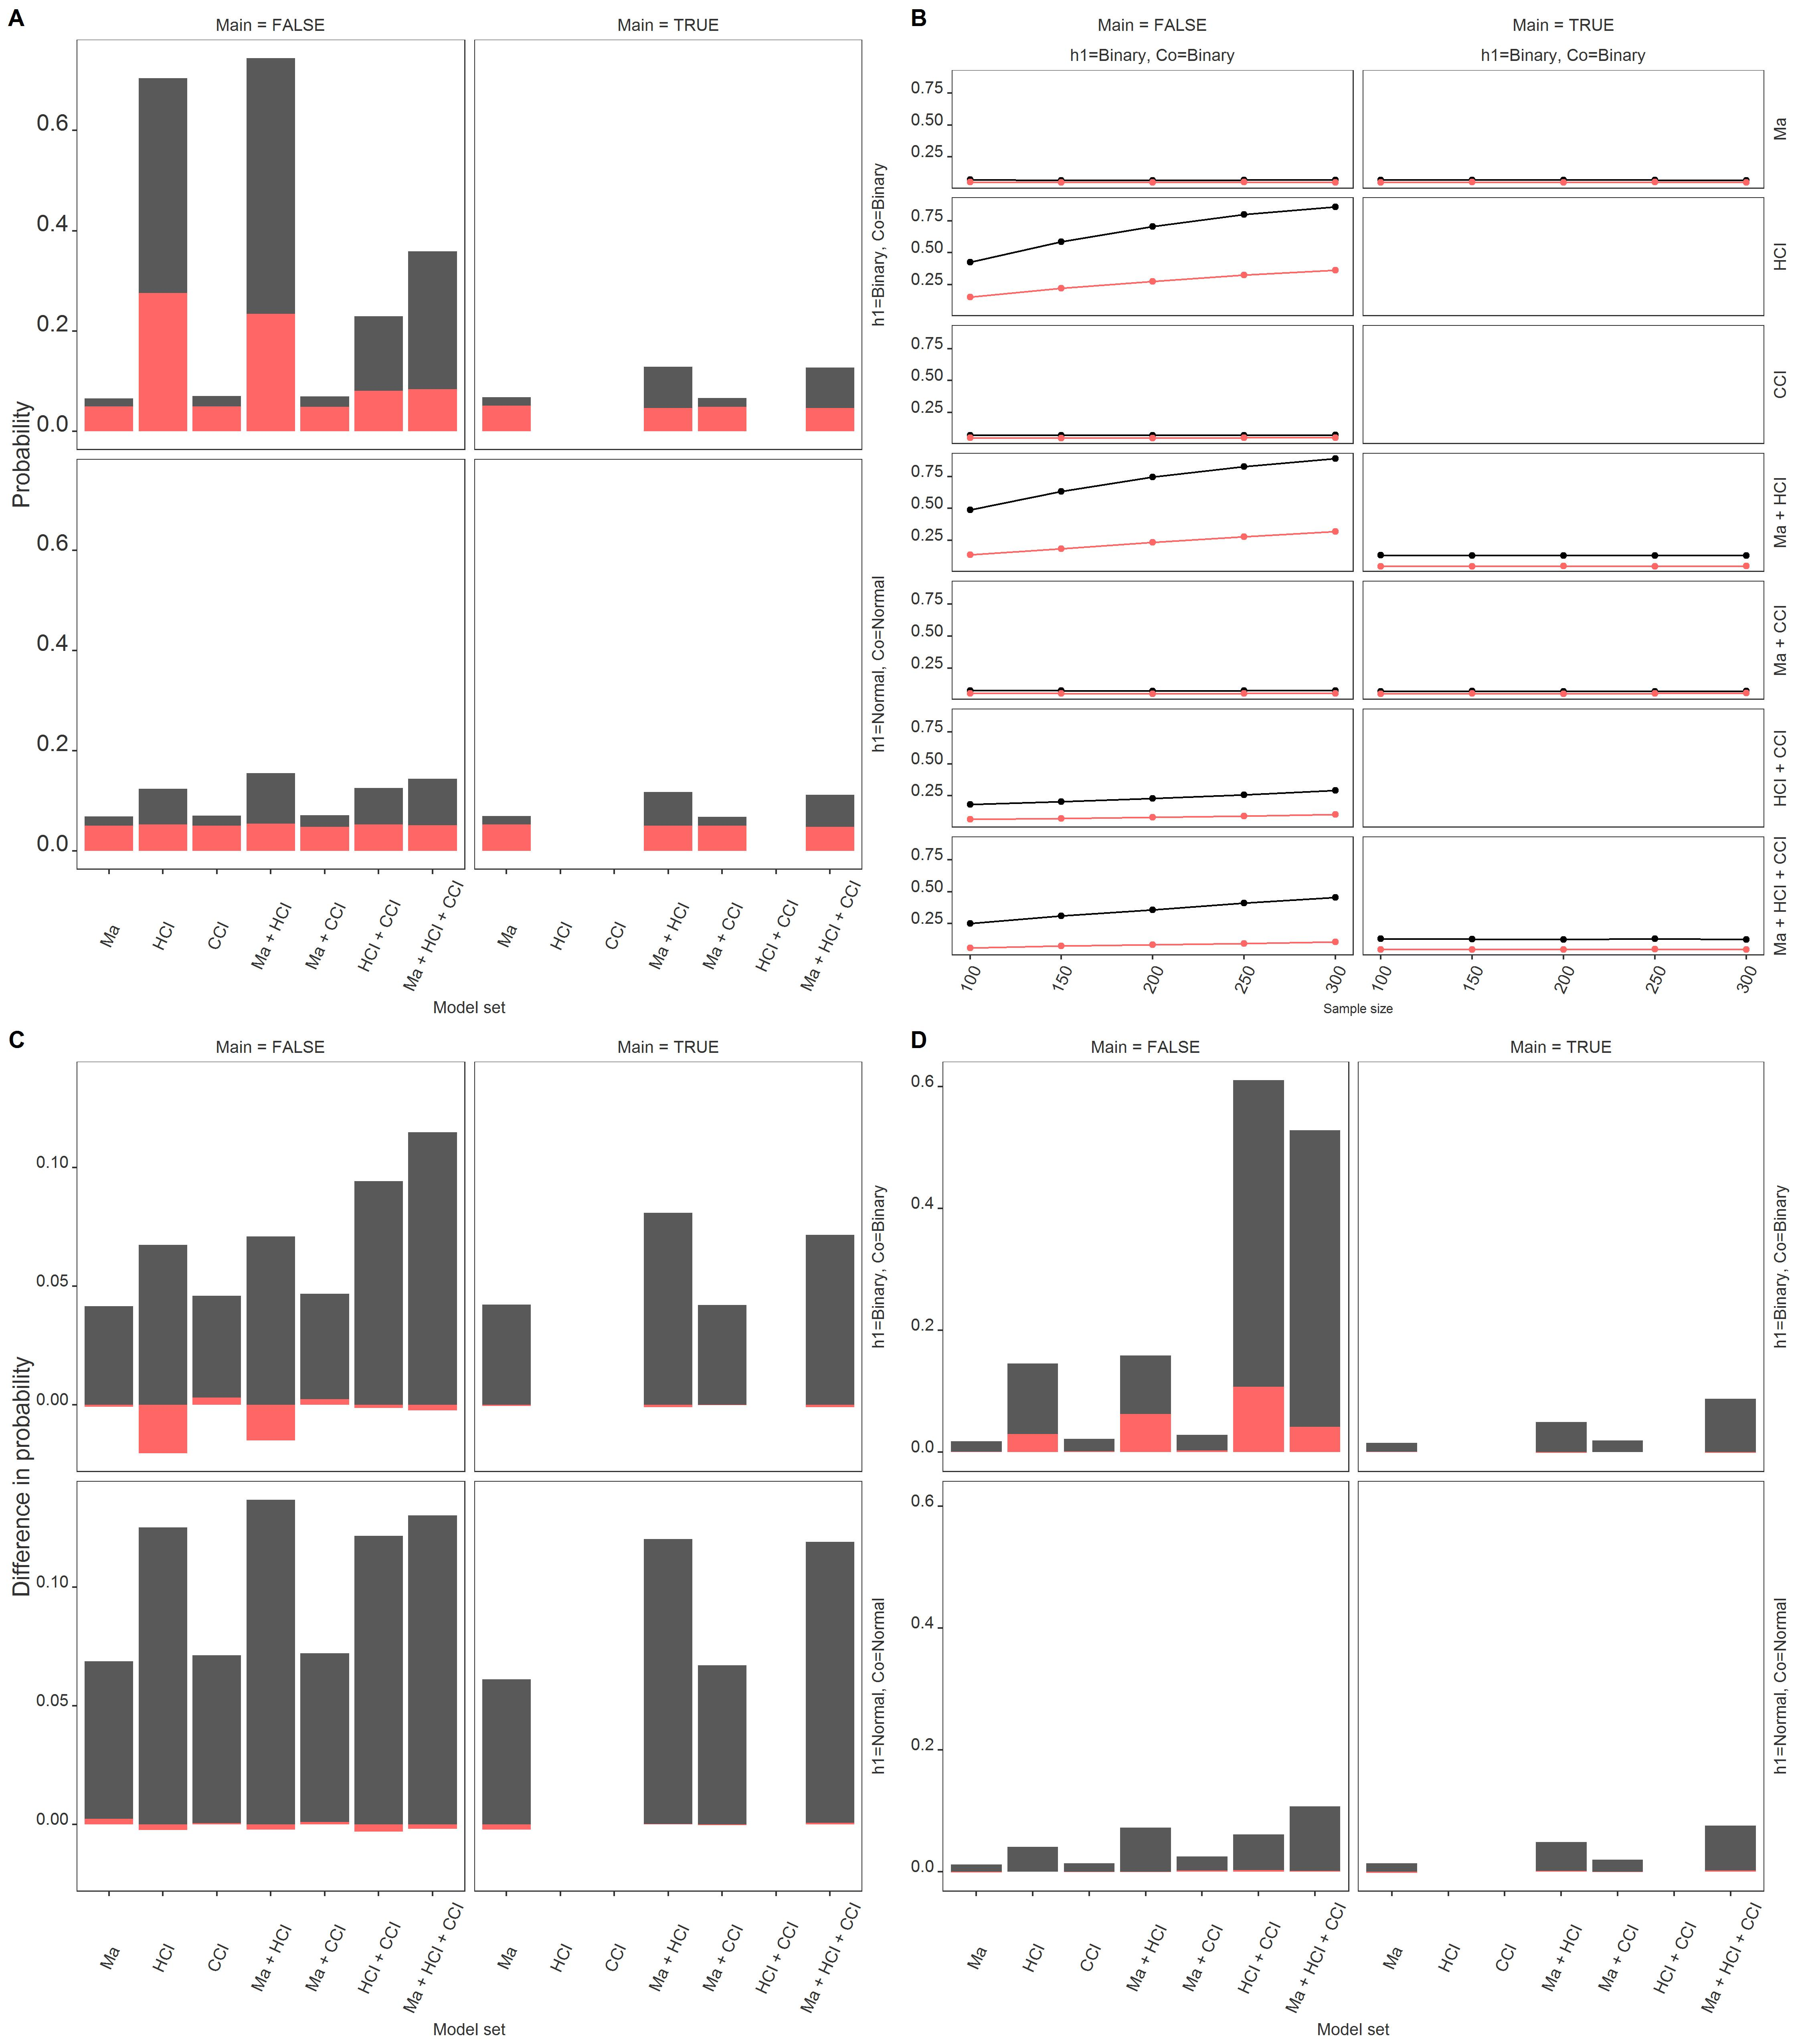
\includegraphics[width=0.8\textwidth]{R/Analysis/Result/Figures/Figure1BF.jpeg}
\centering
\caption{Black is the FPP and red is FPR.  Splitting the false-positive rate by model set and whether the main effects should follow interactions or not. Same figures as Figure 1-4 but with Bonferroni correction}
\label{fig:mainfigure}
\end{figure}